\newpage
\section{Modelli linari}
\subsection{Regression}
Un possibile esempio di regressione potrebbe essere un processo di stima di una funzione di valore
reale sulla base di un insieme finito di campioni rumorosi. Le conoscenze sarebbero $pairs(x, f(x) + random noise)$.\\
La task a questo punto sarebbe trovare $f$ per i dati nella seguente tabella.
\begin{figure}[h!]
    \centering
    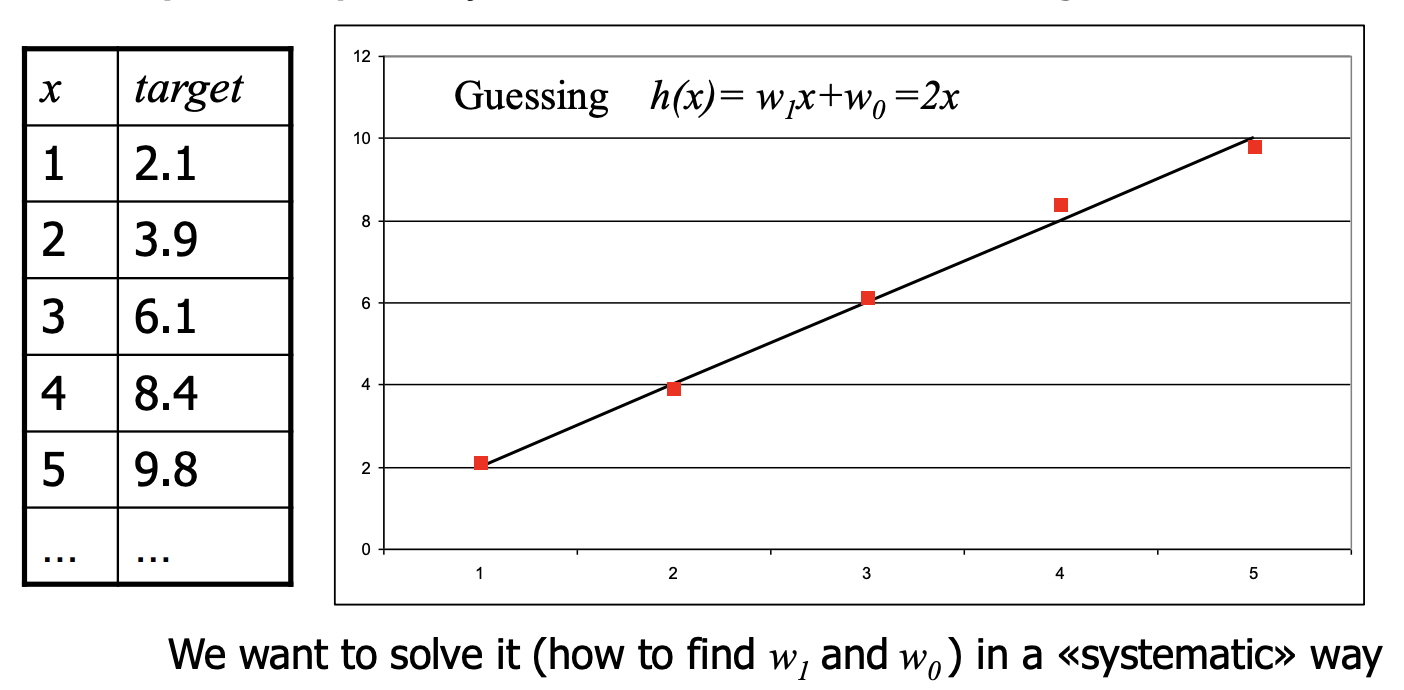
\includegraphics[width=0.65\textwidth]{images/esempio-regresione.png}
\end{figure}
\begin{example}
    Esempio di modelli linari:
    \begin{figure}[h!]
        \centering
        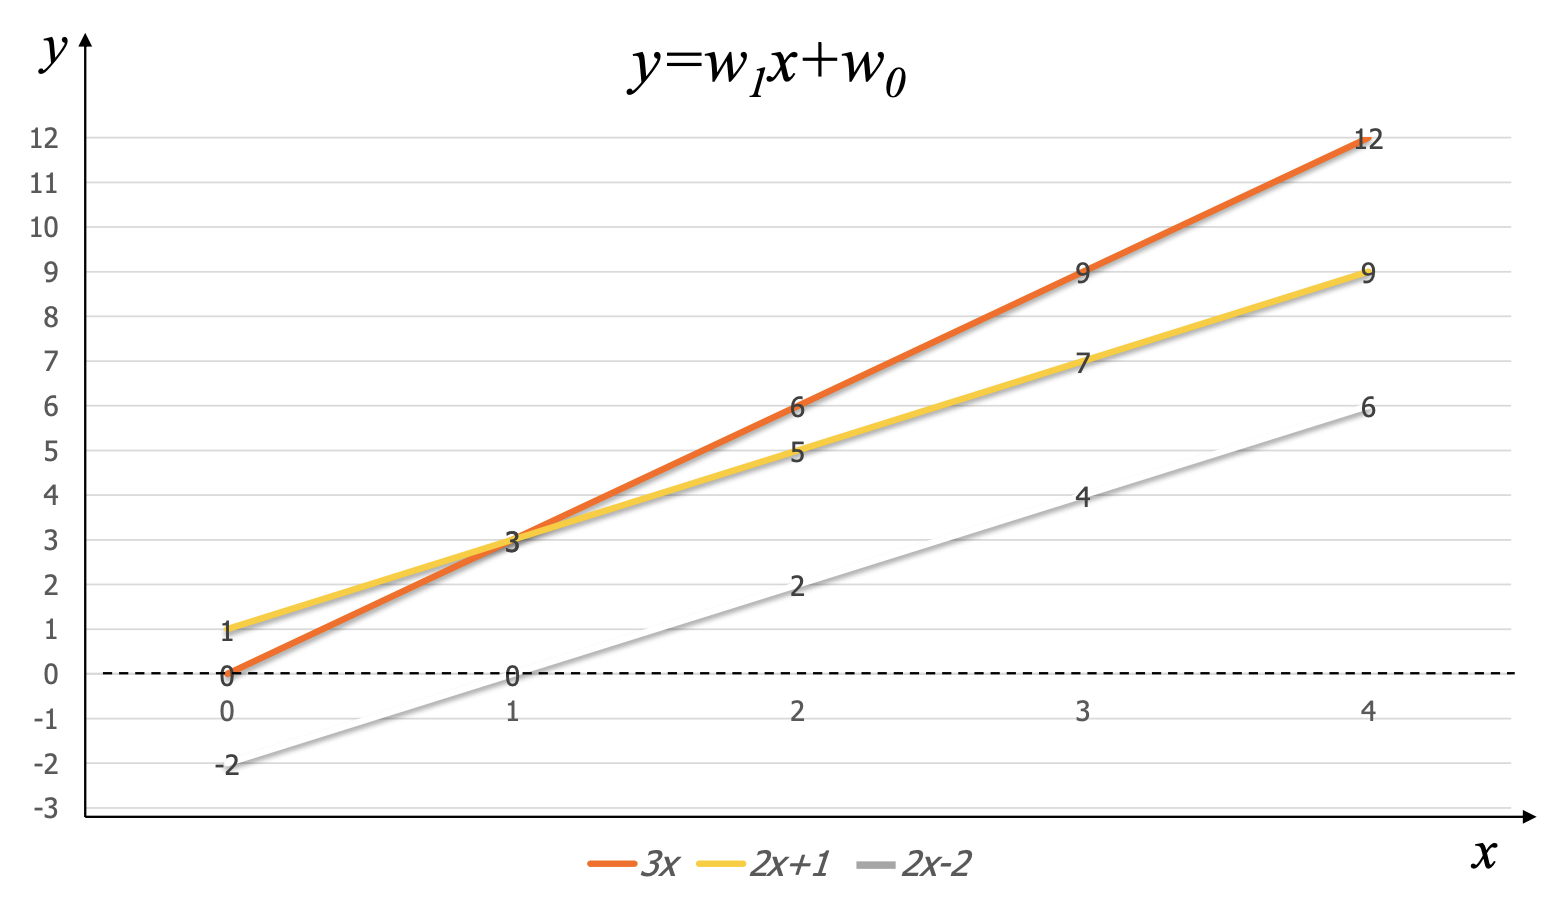
\includegraphics[width=0.65\textwidth]{images/esempio-modelli-lineari.png}
    \end{figure}
\end{example}

\subsubsection{Univariate linear regression}
Il caso univariante, semplice regressione linieare: iniziamo con 1 valore di inputl, $x$ e 
1 valore di output $y$.
\begin{definition}
    Assumiamo che un modello $h_w(x)$ espresso come:
    $$out = h(x) = w_1x + w_0$$
    dove $w$ è il coefficiente a valore reale/paramentro libero (peso).
\end{definition}
Si cerca di avere un adattamento dei dati secondo una “linea retta”. Trovare $h$ (modello lineare) che 
meglio si adattano ai dati (da gli insieme di dati osservati dei valori $x$ e $y$). Assumiamo che la variabile data (y) è (linearmente) 
associata ad un'altra viarialbe (x) o più variabili, da $y = w_1x + w_0 + noise$, dove $w$ è il free par e $noise$ è
un errore misurato al target (con una distribuzione normale). Andiamo a costruire un modello (trovare il valore $w$) per predirre/stimare il prezzo ($y$) dei punti
per altri (osservabile) valori $x$ (prediction).
\begin{figure}[h!]
    \centering
    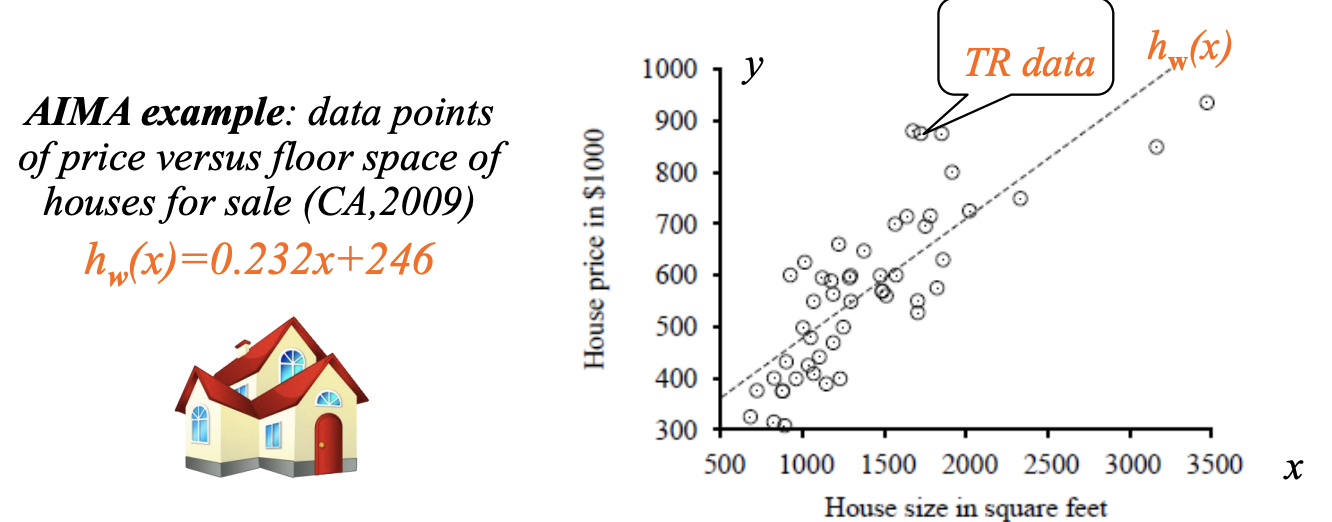
\includegraphics[width=0.55\textwidth]{images/task-model-esempio.png}
\end{figure}
Usiamo poi questi valori per \textbf{predirre/stimare} il prezzo (t) dei punti per altri valore osservabili.
\begin{figure}[h!]
    \centering
    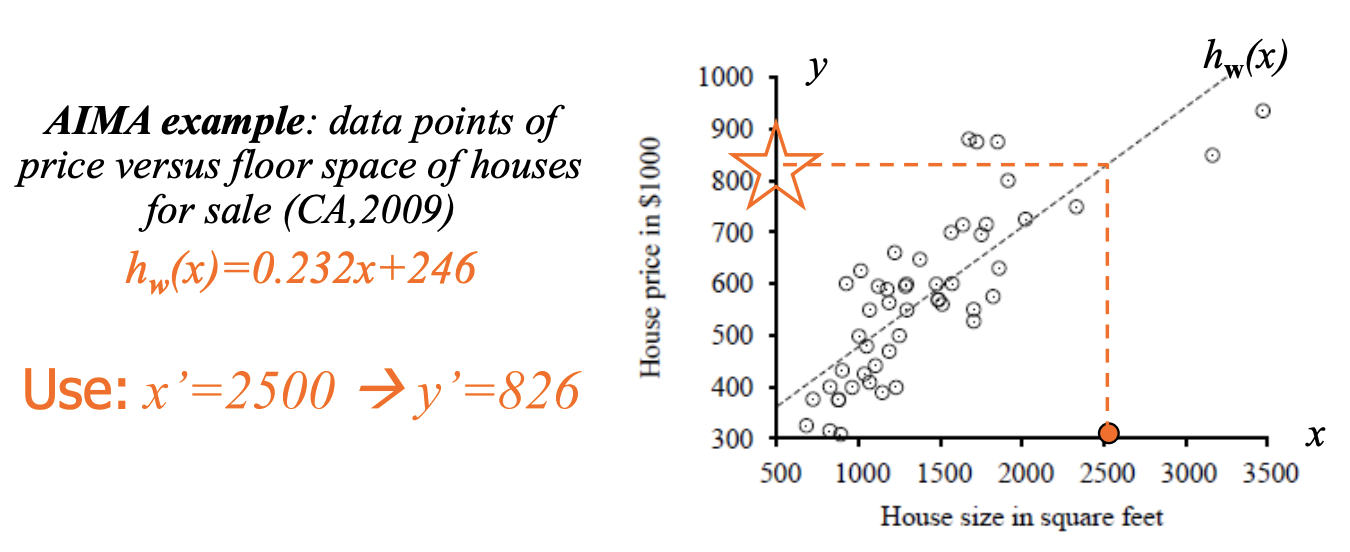
\includegraphics[width=0.55\textwidth]{images/uso-predizione-esempio.png}
\end{figure}

\subsubsection{Learning via LMS}
Abbiamo capito che quindi dobbiamo andare a trovare i valori dei paramentri $w$ ($w_1$ e $w_2$ nei casi univarianti) per andare a minimizzare 
l'output dell'errore del modello (per eseguire un buon fitting). In uno spazio di ipotesi infinito (valore $w$ continuo) abbiamo una buona soluzione
data dalla matematica classica, possiamo "imparare" da dei semplici tools, sebbene semplice incluse moltri concetti rileventi per
il ML moderno ed è alla abse dei metodi evoluti in the field. Definiamo qui una \textbf{funzione less / error} e usiamo il \textbf{Least Mean Square (LMS)} approccio.\\\\
\textbf{Il training} si fa trovando $w$ tale che minimizzi l'\textbf{errore}/la \textbf{perdita epirica} (il miglior dato che fitta nel training set con l'esempio $l$)

\begin{definition}
    Andiamo allora a definire LMS con:
    \begin{itemize}
        \item \textbf{Given} un insieme ti esempi di training $l$ ($x_p, y_p$) $p = 1 \dots l$
        \item \textbf{Trovare} $h_w(x)$ nella forma $w_1 x + w_0$ (quindi i valori di $w$) che minimizzano la perdita attesa dei dati di training.
    \end{itemize}
    Per la perdita usiamo la radice dell'errore.\\
    Da qui il \textbf{least (mean) square} si tratta di trovare la $w$ che minimizzi la somma residua delle ragdici [$argmin_w Error(w) in L_2$]
    $$Loss(h_w) = E(w) = \sum_{p=1}^{l} (y_p - h_w(x_p))^2 = \sum_{p=1}^{l}(y_p - (w_1 x_p + w_0))^2$$
    Dove $x_p$ è $p-th$ input/pattern/esample, $y_p$ l'output per $p$, $w$ free par., $l$ numero degli esempi.
\end{definition}
\hspace{-15pt}Perché usare LMS per adattarsi ai dati con $h$? Il \underline{least (mean) square} trova $w$ per minimizzare la \textbf{somma di radici residua} [$argmin_w Error(w) \in L_2$]:
\begin{figure}[h!]
    \centering
    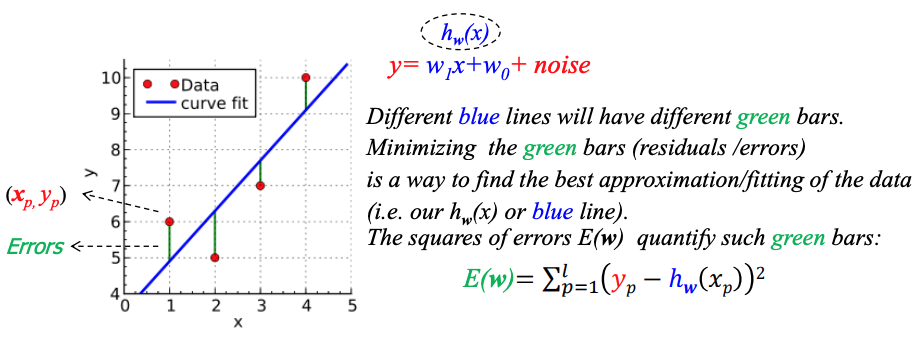
\includegraphics[width=0.6\textwidth]{images/lms.png}
\end{figure}

\hspace{-15pt}Il metodo dei minimi quadrati è un approccio standard alla soluzione approssimata di sistemi sovradeterminati, cioè insiemi di equazioni
in cui ci sono più equazioni che "sconociuti".\\\\
\textbf{Come si risolve?} Ricorda che il minimo locale è un punto stazionario, il gradiente è nullo.
$$\frac{\partial E(wi)}{\partial w_i} = 0 \hspace{15pt} i = 1, \dots, dim\_input + 1$$
Per una semplice regressione lineare (2 paramentri liberi) abbiamo che:
$$\frac{\partial E(w)}{\partial w_0} = 0 \hspace{15pt} \frac{\partial E(w)}{\partial w_1} = 0$$
Funzione di perdita convessa $\Rightarrow$ abbiamo la seguente soluzione (senza minimo locala).
$$w_1 = \frac{\sum x_p y_p - \frac{1}{l}\sum x_p \sum y_p}{\sum x_p^2 - \frac{1}{l} (\sum x_p^2)} = \frac{Conv[x, y]}{Var[x]}, \hspace{10pt} w_0 = \overline{y} - w_1 \overline{x} \hspace{20pt} \overline{y} = \frac{1}{l}\sum_{p \to 1} t_p  \hspace{7pt} \overline{x} = \frac{1}{l}\sum_{p\to 1}x_p$$
Calcolare il gradiante per 1 (ciascuno, omettendo quindi $p$ per $x$) pattern p. 
$$\frac{\partial E}{\partial w_i} = \frac{\partial (y - h_w(x))^2}{\partial w_i} = 2(y - h_w(x))\frac{\partial (y - h_w(h))}{\partial w_i} = 2(y - h_w(x))\frac{\partial (y - (w_1 x + w_0))}{\partial w_i}$$

\subsection{Summarizing}
\begin{itemize}
    \item \textbf{Given} un insieme di $l$ esempi di training ($x_p, y_p$) ed una funzione di perdita.
    \item \textbf{Find} il valore del peso $w$ per costruire $h_w(x)$ espresso come $y/out = w_1 x + w_0$ (minimizzare la perdita attesa dei dati di training)
\end{itemize}
\begin{figure}[h!]
    \centering
    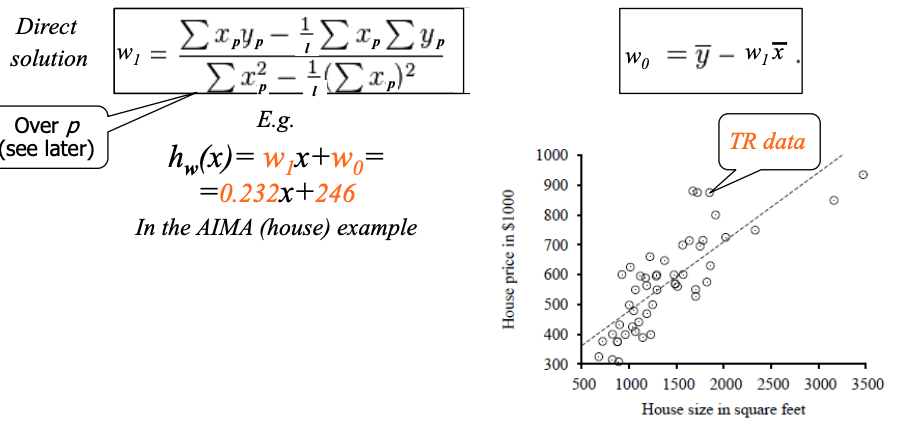
\includegraphics[width=0.55\textwidth]{images/summarizing.png}
\end{figure}
Ora è possibile usarlo per nuovi $x'$ per predirre $y'$. Vediamo ora un approccio differente.

\subsection{Gradiant descent (ricerca locale)}
Errore delle superfici per il linear model con 2 pesi. Parabolico per $E(w) = E([w_0, w_1]^T)$ (funzione quadratica convessa)
\begin{figure}[h!]
    \centering
    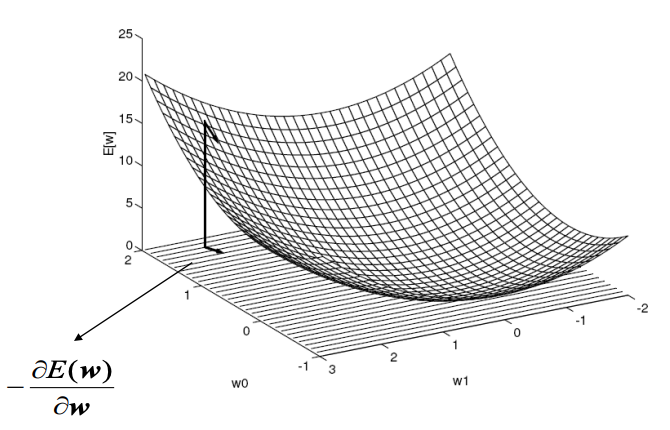
\includegraphics[width=0.4\textwidth]{images/error-surface.png}
\end{figure}

\hspace{-15pt}Spazio ipotetico con 2 parametri $w_0, w_1$. Il gradiente di $E(w)$ è il nostro "compasso" per trovare il minimo.\\\\
La derivazione precedente suggerisce la linea per costruire un \textbf{algoritmo iterativo} basato su $\frac{\partial E(w)}{\partial w_i}$
\begin{definition}
    \textbf{Gradiente} = direzione salita, possiamo muoverci verso il minimo con un gradiente in discesa ($\Delta w =$ gradiente di $E(w)$)
\end{definition}
\begin{definition}
    \textbf{ricerca locale} inizia con vettore di pesi iniziali. Esso viene modificato iterativamente per diminuire
    fino a minimizzare la funzione di errore (discesa più ripida).
    $$w_new = w + \eta \cdot \Delta w$$
    Dove $\eta$ è una constante (step size) chiamata \textbf{learning rate}
\end{definition}
\begin{figure}[h!]
    \centering
    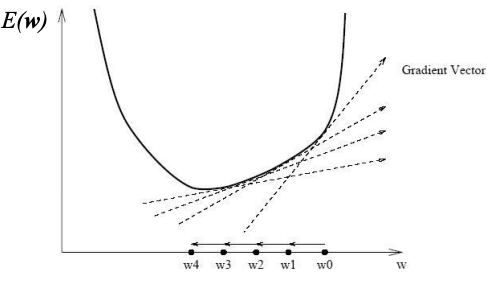
\includegraphics[width=0.5\textwidth]{images/gradieant-descent.png}
\end{figure}
Le motivazioni intuitive del gradiant descent sono che dalla formulazione, $w_new = w + \eta \cdot \Delta w$ possiamo ottenere:
$$\Delta w_0 = -\frac{\partial E(w)}{\partial w_0} = 2(y- h_w(x)) \hspace{15pt} \Delta w_1 = -\frac{\partial E(w)}{\partial w_i} = 2(y - h_w(x)) \cdot x$$
\begin{definition}
    Questa è una "error correction rule" chiamata \textbf{delta rule} che cambia la proporzione $w$ con l'errore (target-output):
    \begin{itemize}
        \item (target y - output) = err  = 0 $\to$ nessuna correzione 
        \item output > target $\to$ (y - h) < 0 (output troppo alto)
        \begin{itemize}
            \item Se $\Delta w_0$ negativo $\to$ si riduce $w_0$ e 
            \item if (input $x > 0$) $\Delta w_1$ negativo $\to$ si ricude $w_q$ else si aumenta $w_1$
        \end{itemize}
        \item output < target $\to$ $(y - h) > 0$ (output è troppo lento)
    \end{itemize} 
\end{definition}
\hspace{-15pt}In questo modo andiamo a migliorare l'apprendimento dai precedenti errori.\\\\
In conclusione possiamo dire che l'approccio del Gradiant descent è semplice ed efficacie per ricerca locale e approcci alla soluzione LMS, inoltre
ci permette di cercare in uno spazio infinito di ipotesi, può essere facilmente applicato sempre per $H$ contuno e perdite differenziabili non solo ai modelli lineari
(ess. reti neurali e deep learning models). A livello di efficienza molti miglioramenti sono possibili come il Newton's method, Conjugate Gradiant.

\subsection{Estensioni a $l$ dati}
\begin{definition}
    Possiamo riassumente per $l$ patterns $(x_p, y_p)$ nel seguente modo.
    $$\Delta w_0 = - \frac{\partial E(w)}{\partial w_0} = 2 \sum_{p=1}^{l}(y_p - h_w(x_p)) \hspace{15pt} \Delta w_1 = -\frac{\partial E(w)}{\partial w_1} = 2 \sum_{p=1}^{l}(y_p - h_w(x_p)) \cdot x_p$$
    Dove $x_p$ è un p-esmo input, $y_p$ l'output per $p$, $w$ una coppia libera, $l$ numero di esempi.
\end{definition}
\hspace{-15pt}Possiamo aggiornare $w$ dopo (ripetendo) una fase di dati di training $l$ $\to$ \textbf{algoritmo di batch} (blu). Oppure
possiamo aggiornare $w$ dopo ogni pattern $p \to$ \textbf{on-line algorithm} (discesa del gradiente stocastico) (purple and green), questo caso 
potrebbe essere più veloce, ma necessitare di step più piccoli.

\subsection{Estendere a vettori di input}
Questo è una caso standard, usare da 2 finoa centinaia di variabili/features di input  $x = [x_1, x_2, \cdots, x_n]$, il \textbf{pattern} di input
è un vettore.
\begin{example}
    Degli esempi potrebbero essere calcolare lo stato di una scacchiera in un gioco di dama per num. di pezzi bianchi/neri/re/catturati
    nel turno successivo: 6 variabili. $w$ peso che viene dalle "fetures sul tavolo".
\end{example}
\hspace{-15pt}Facciamo un piccolo riassunto della notazione per i dati. Prendiamo una $X$ matrice $l, x, n$ dove $l$ sono le righe
mentreh $n$ le colonne (feuteres, variabili, attributi), $p = 1, \cdots, l$ e $i = 1, \cdots n$. Abbiamo spesso bisogno di omettere alcuni
indici quando il contesto è chiaro, ad es:
\begin{figure}[h!]
    \centering
    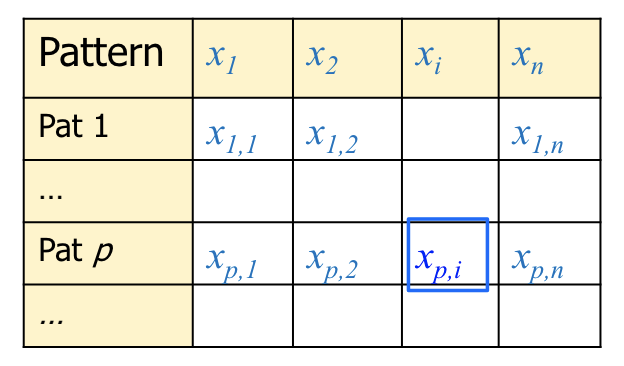
\includegraphics[width=0.5\textwidth]{images/resume-data-notation.png}
\end{figure}
\begin{itemize}
    \item Ogni riga, $x$ generica (vettore in grassetto), un raw nella tabella: (input) esempio, pattern, instance, sample, ..., input vector, ...
    \item $x_i$ o $x_j$ (scalari): componenti $i$ o $j$ (dato un pattern, omettendo p).
    \item $x_p$ (o $x_i$) (vettor in grassetto) il p-esimo (o i-esimo) raw nella tabella = pattern $p$ (o i)
    \item $x_p,i$ (scalare) anche come ($x_p$): componente $i$ nel pattern $p$ (o usamo $x_p,j$ per il componente j, ecc.)
    \item Per il target sono solitamente usiamo solo $y_p$ con $p=1, \cdots l$ (lo stesso per $d$ o $t$)
\end{itemize}
Per la notazione di input multidimensionali andiamo ad assumere una colonna vettere per $x$ e $w$ (in grassetto). Numero 
del dato $l$, dimensione del vettore di input $n$, $y_p$ (targets) e $p = 1, \cdots, l$
$$w^t x + w_0 = w_0 + w_1 x_1 + w_2 x_2 + \cdots w_n x_n = w_0 + \sum_{i=1}^{n} w_i x_i$$
\begin{note}
    Notare che spesso, come prima, la notazione di trasposta $T$ in $w^T$ è omessa.
\end{note}
\hspace{-15pt}$w_0$ è l'intercetta, la soglia, il bias, l'offset.. Spesso è conveninente per includere la constante $x_0 = 1$ 
in modo che possiamo scriverlo come:
$$w^T x = x^T w (inner product) \hspace{15pt}x^T = [1, x_1, x_2, \cdots, x_n] \hspace{15pt} w^t = [w_0, w_1, w_2, \cdots, w_n]$$
\begin{note}
    Notare che $w$ è un parametro (libero) continuo "pesi".
\end{note}
\newpage
\hspace{-15pt}In una vista geometrica avremmo quello che si chiama \textbf{iperpiano}. Per 2 variabili avremmo:
$$x^T w = w^T x = w_0 + w_1 x_1 + w_2 x_2 \hspace{20pt} \text{(n dim)} w^t = [w_0, w_1, w_2, \cdots, w_n]$$
\begin{figure}[h!]
    \centering
    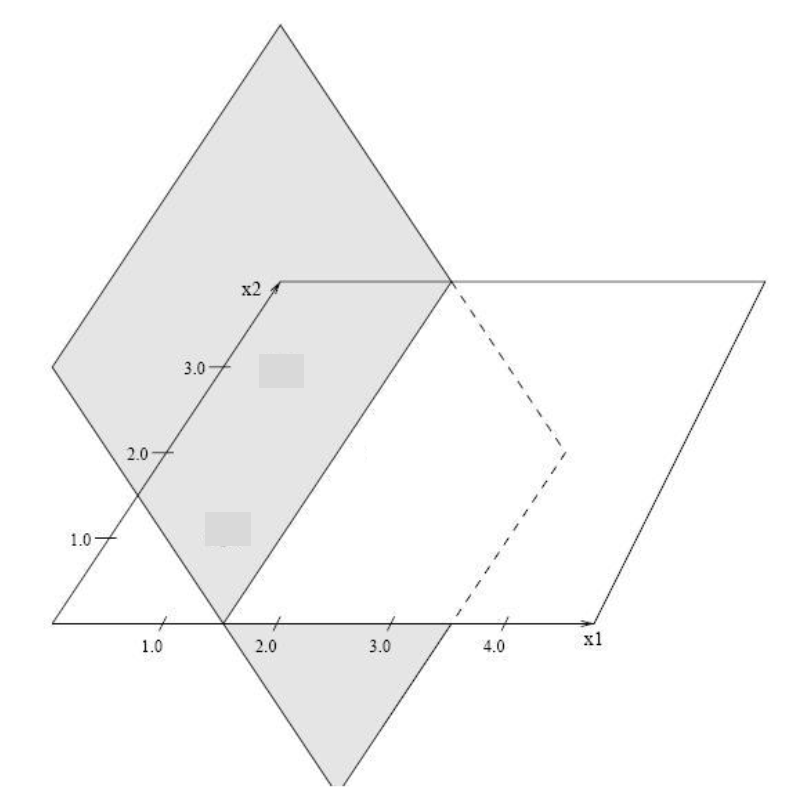
\includegraphics[width=0.2\textwidth]{images/hyperplane.png}
\end{figure}
Quindi possiamo definirlo come:
$$h(x_p) = x_p^T w = \sum_{i=0}^{n}x_{p,i} w_i$$
Possimao sintetizzare il caso con input di dimensione n, e l patterns nel seguenti modo:
\begin{itemize}
    \item \textbf{Given} un insieme di $l$ esempi di trainign $x_p, y_p$
    \item \textbf{Find} il peso del vettore $w$ che minimizzi la perdita attesa dei dati di training.
\end{itemize}
$$E(w) = \sum_{p=1}^{l}(y_p - x_p^T w)^2 = ||y - Xw||^2$$
Dove $x_p$ è il p-esimo input del vettore, $y_p$ è l'outpu per p, $w$ è la coppia libera, $l$ il numero
di esempi e $n$ la dimensione dell'input.

\subsection{Algoritmo iterativo di discesa del gradiante}
\begin{definition}
    Definiamo ora \textbf{l'algoritmo iterativo di discesa del gradiante}
    $$\Delta w_i = -\frac{\partial E(w)}{\partial w_i} = \sum_{p=1}^{l}(y_p - h_w(x_p)) \cdot x_{p,i} = w\sum_{p=1}^{l}(y_p - x_p^T w)x_{p,i}$$
    Abbiamo che il 2 è una costante che può essere ignorata nello sviluppo dell'algoritmo, mentre $x_{p,i}$ è il componente $i$ del pattern $p$
\end{definition}
\hspace{-15pt}Questo è una estensione vettoriale al gradiente molto semplice nel quale ogni x, ha il suo $w_i$ e il suo $\Delta w_i$ (come il singolo x prima).
Il vettore di gradianti per una dimensione n sarebbe il seguente:
$$
\Delta w = -\frac{\partial E(w)}{\partial w} = 
\begin{bmatrix}
    -\frac{\partial E(w)}{\partial w_1}\\
    -\frac{\partial E(w)}{\partial w_2}\\
    -\frac{\partial E(w)}{\partial w_i}\\
    \cdots\\
    -\frac{\partial E(w)}{\partial w_n}
\end{bmatrix}
= 
\begin{bmatrix}
    \Delta w_1\\
    \Delta w_2\\
    \Delta w_i\\
    \cdots \\
    \Delta w_n
\end{bmatrix}
$$
Possiamo lavorare in uno spazio a più luci senza la necessità di visualizzarlo. PS $w_0$ viene omesso sopra, puoi includerlo facilmente.\\\\
Per riassumenre possiamo spiegare l'algorimo in dei semplici passaggi:
\begin{enumerate}
    \item Iniziare con un vettore dei pesi $w_initial$ (piccolo), fissando un $\eta$ ($0 < \eta < 1$).
    \item Calcolare $\Delta w =$ -"gradiante di $E(w)$" = $-\frac{\partial E(w)}{\partial w}$ (o per ogni $w_j$)
    \item Calcolare $w_new = w + \eta \cdot \Delta w$ (o per ogni $w_j$) 
    \item Ritornare al 2 e ripetere finché non si converge o $E(w)$ è "sufficetemente piccolo"
\end{enumerate}
$\Delta w/l$ least mean square:
\begin{itemize}
    \item Batch versions ($\Delta w$ dopo ogni "epoch" dei dati "l")
    \item Stochatic/on-line version: aggiornare w per ogni pattern p (da $\Delta_p w = x_p (y_p - x_p^T w)$ senza aspettare la somma totale su $l$)
    \item $\eta$ = learning rate: seed/stabilty trade-off: può essere (gradualmente) decrementato a zero (garantendo convergenza, 
    evitando oscillazioni intorno al min.)
\end{itemize}
\begin{figure}[h!]
    \centering
    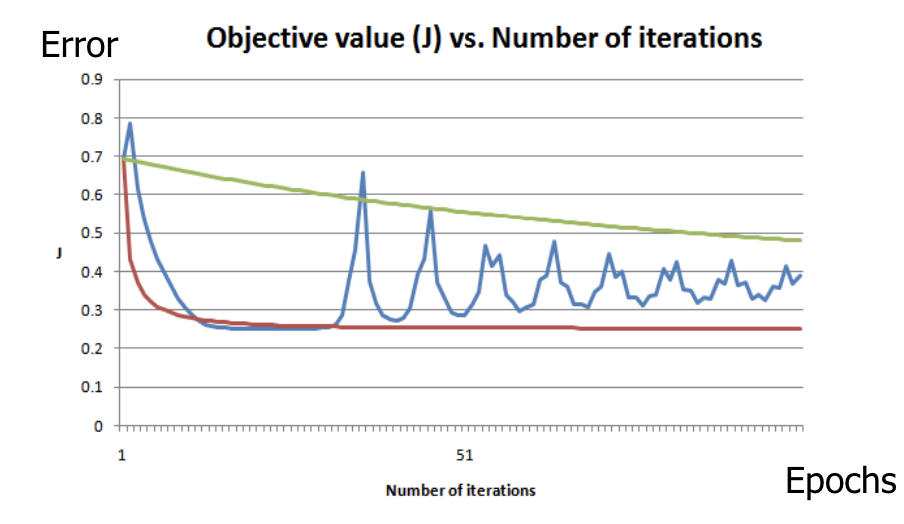
\includegraphics[width=0.6\textwidth]{images/learning-curve-examples.png}
\end{figure}
\begin{definition}
    Queste sono le \textbf{curve di apprendimento}: Mostrano come si verifica l'errore diminuisce attraverso il gradiente iterazioni di discesa.
\end{definition}
I vantaggi dei modelli lineari sono che se funzionano bene sono un modello fantastici: molto semplice,
tutte le informazioni dei dati sono in $w$, facili da interpretare, dati "rumorosi" sono accettati, Fenomeni lineari: un sogno per la scienza: ideale per realizzare un fenomeno “naturale”.
legge.

\subsection{Limitazioni}
Una delle limitazioni dei modelli lineari sono le tasks di regressione per problemi non lineari.
\begin{figure}[h!]
    \centering
    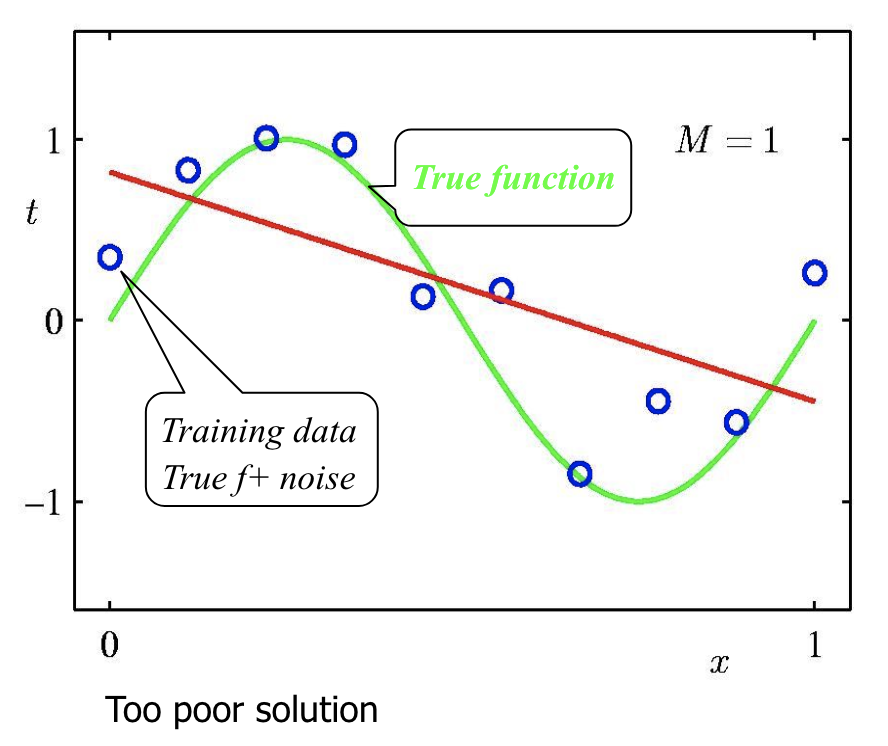
\includegraphics[width=0.3\textwidth]{images/regression-task-non-linear-problems.png}
\end{figure}

\hspace{-15pt}Proviamo ora a muoverci verso delle relazioni non-lineari. Notare che in $h_w(x) = w_1 x + w_0$ o $h_w(x) = w^T \cdot x$ 
come modelli statistici parametrici: "\textbf{lineare}" non si riferisce a questa linea rette, piuttosto al modo in cui
si verificano i coefficienti di regressione $w$ nell'equazione di regressione.\\\\
Possiamo quindi utilizzare anche input trasformati, come ad esempio $x, x^2, x^3, x^4, \cdots$ con una relazione \textbf{non lineare} input e outpout, 
gestiamo la macchina di learning (Least Square solution) sviluppandola nel seguente modo:
$$h_w(x) = w_0 + w_1 x + w_2 x^2 + \cdots + w_Mx^M = \sum_{j=0}^{M}w_j x^j$$
Detta \textbf{polynomial regression}.
\newpage
\begin{example}
    Facciamo un esempio non-lineare.
\end{example}
\begin{wrapfigure}[10]{r}{0.4\textwidth}
    \vspace{-25pt}
    \centering
    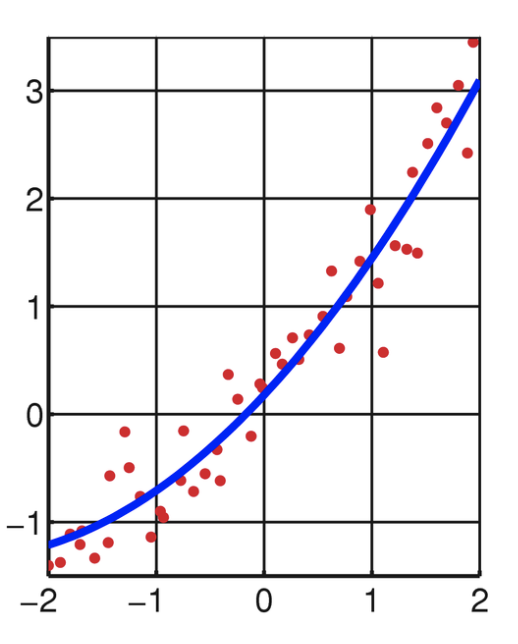
\includegraphics[width=0.2\textwidth]{images/esempio-non-lineare.png}
\end{wrapfigure}
Il risultato dell'adattamento di una funzione quadratica (in blu) $M=2$, passante un insieme di punti dati (in rosso). \\\\
Nei minimi quadrati lineari la dunzione non deve essere lineare in argomento (varibili di input) ma solo nei parametri ($w$) che sono
determinati per dare il best fit.

\subsection{Linear basis expansion}
Una generalizazzione (che mostriamo per la regressione) è la \textbf{LBE} o \textbf{linear basis expansion}, che definiamo come
$$h_w(x) = \sum_{k=0}^{K}w_k\phi_k(x)$$
L'argomento di input è un vettore con variabili aggiuntive, le quali sono trasformazioni di $x$ secondo una funzione $\phi$ ($\phi_k: R^n \to R$).
\begin{example}
    Alcuni eesempi sono:
    \begin{itemize}
        \item Rappresentazione polinomiale $x: \phi(x) = x_j^2$ o $\phi(x) = x_jx_i$ ...
        \item Trasformazione non lineare di un singolo input $\phi(x) = \log(x_k), \phi(x) = root(x)$, ...
        \item Trasformazione non lineare di input multipli: $\phi(x) = ||x||$
        \item Splines, ...
    \end{itemize}
\end{example}
\hspace{-15pt}Il numero di paramentri $K>n$. Il modello è lineare nei paramentri (anche in $\phi$, non in $x$): possiamo usare lo stesso
algorimo di learning di prima.

\begin{example}
    [1-dim $x$] \hspace{15pt} $\phi_j(x) = x^j$.
    $$h(x) = w_0 + w_1x + w_2x^2 + \dots + w_Mx^M = \sum_{j=0}^{M}w_jx^j$$
    1-dim regressione polinomiale ($K=M$). Per il numero di termini nel polinomio con D dim. input vedremo più avanti.\\\\
    O "qualsiasi altro" $\phi(x) = \phi([x_1, x_2, x_3])$
    $$h(x) = w_1x_1 + w_2 x_2 + w_3 \log(x_2) + w_4\log(x_3) + w_5(x_2x_3) + w_0$$
\end{example}
\hspace{-15pt}Vediamo ora le criticità (sia positive che negative) del basis expansion, per poi arrivare 
ai così detti approcci "\textbf{dizionari}".
\begin{itemize}
    \item \textbf{PROS}: È più espressivo: può modellare in modo più complicato
    relazioni (rispetto a quelle lineari).
    \item \textbf{CONS}: Con un'ampia base di funzioni, abbiamo bisogno di metodi per
    controllare la complessità del modello.
\end{itemize}
$$h_w(x) = w_0 + w_1x + w_2x^2 + \dots + w_Mx^M = \sum_{j=0}^{M}w_jx^j$$
\newpage
\begin{figure}[h!]
    \centering
    \begin{subfigure}{.3\textwidth}
        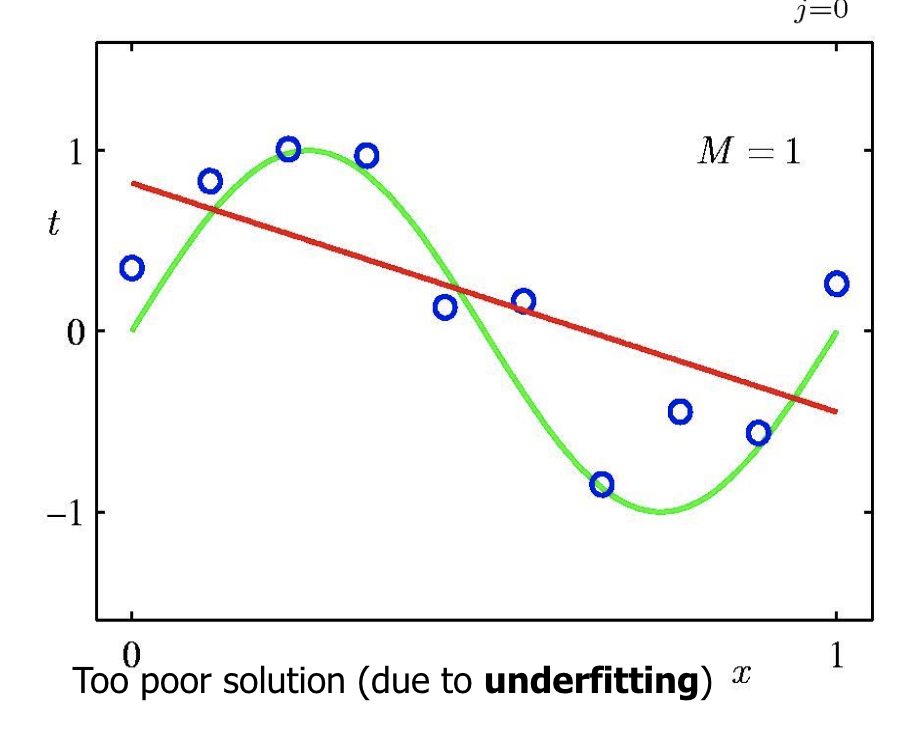
\includegraphics[width=\textwidth]{images/1st-order-polynomial.png}
        \caption{1st order polynomial}
    \end{subfigure}
    \begin{subfigure}{.3\textwidth}
        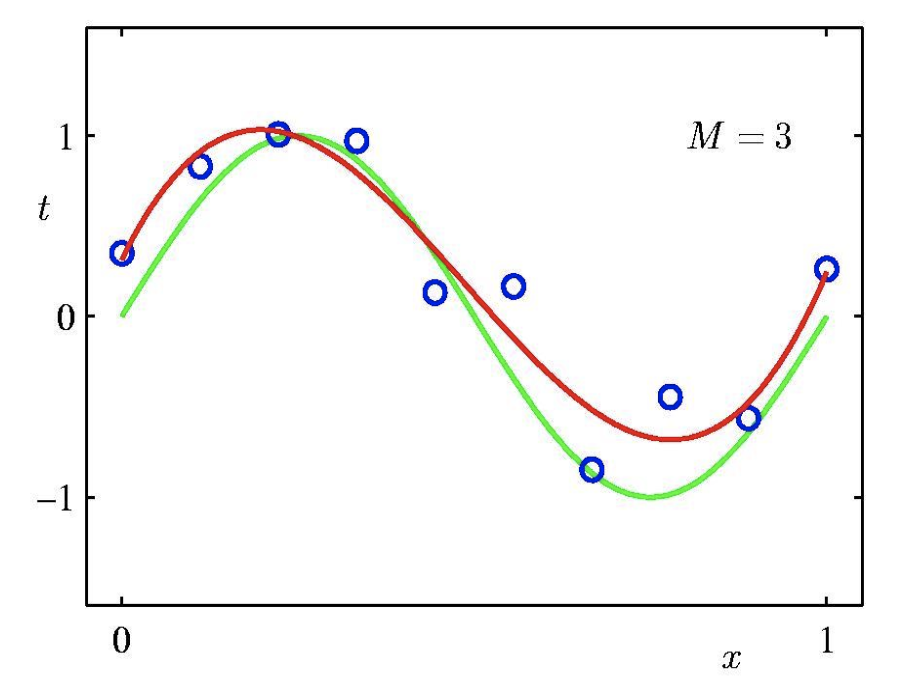
\includegraphics[width=\textwidth]{images/3st-order-polynomial.png}
        \caption{3st order polynomial}
    \end{subfigure}
    \begin{subfigure}{.3\textwidth}
        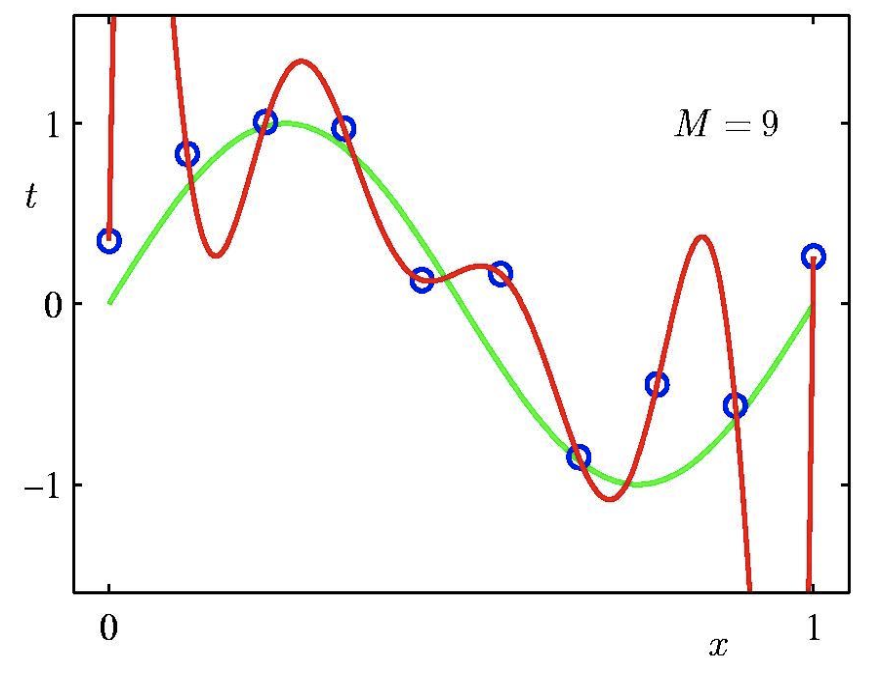
\includegraphics[width=\textwidth]{images/9st-order-polynomial.png}
        \caption{9st order polynomial}
    \end{subfigure}
\end{figure}

\hspace{-15pt}Notiamo che l'ultimo caso è molto più flessibile, ma potrebbe essere eccessivo. $E(w) = 0$ nei dati di training, diventa
un modello tropp complesso, scarsa rappresentazione della funzione vera (verde) (a causa del sovradattamento).\\\\
Capiamo dunque che il tradeoff della complessità è che:
\begin{itemize}
    \item Un modello troppo semplice: non fitta i dati in modo corretto \textbf{underfitting}
    \item Un modello troppo complesso: Altamente sensibile alle leggere perturbazioni dei dati \textbf{overfitting}
\end{itemize}
Vuoi scegliere la regolarizzazione per bilanciare i due casi attraverso il controllo della complessità del modello (intesa come flessibilità).
Considerando che la complessità non è dovuta al costo computazionale ma a misura della flessibilità del modello per adattarsi ai dati.

\subsection{Regularization}